\textbf{Входные параметры:}
  
x --- действительное число, для которого считаем функцию принадлежности.
 
a --- левая крайняя граница;
 
b --- начало устойчивой области;
 
с --- конец устойчивой области;
 
d --- правая крайняя граница.

m --- функция принадлежности не может быть выше этого значения [0;1].

\textbf{Возвращаемое значение:}
 
Значение функции принадлежности.

\textbf{Формула:}
\begin{equation*}
f\left(x \right)=\min\left(m, \left\lbrace \begin{aligned}  0,& \text{ если } x < a   ; \\\dfrac{x-a}{b-a},& \text{ если } x \in \left[ a; b\right)   ; \\1,& \text{ если } x \in \left[ b; c\right] ; \\\dfrac{d-x}{d-c},& \text{ если } x \in \left( c; d\right]   ; \\ 0,& \text{ если } x >d. \end{aligned}\right.\right) 
\end{equation*}

 \begin{figure} [h] 
   \center
   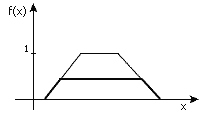
\includegraphics {MHL_TrapeziformTruncatedFuzzyNumber_Graph.png}
   \caption{График функции} 
   \label{img:MHL_TrapeziformTruncatedFuzzyNumber_Graph}  
 \end{figure}
